\section{Style transformation using autoencoder}
As the project evolved we also wanted to achieve the style transformation of songs. For this purpose we created an autoencoder, that uses the Hilbert curve data preprocessing method. The idea was that if we teach our network with piano music only, it would learn how to restore piano music from the bottleneck. Our expectation was that after the learning is complete, if we use the autoencoder on non piano based music (in our case guitar) the network would transform the non piano input to piano music, since it only knows how to restore waves/amplitudes specific only to pianos. This was more or less achieved as you will possibly hear in our presentation, we believe that by fine-tuning the network (increase complexity while decreasing the bottleneck) it might be able to produce real, comfortable to listen to, piano transformed music.

\ref{fig:auto}
\begin{figure}[H]
	\centering
	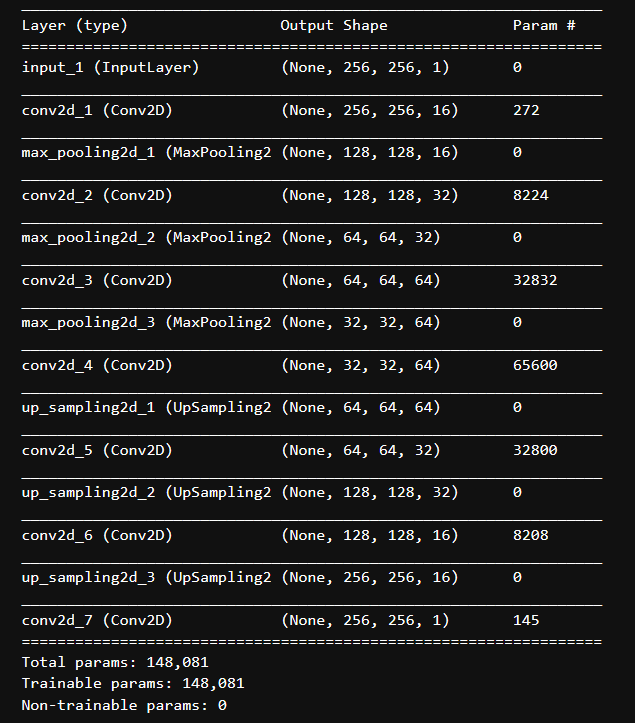
\includegraphics[width=\linewidth]{auto_arch.png}
	\caption{Autoencoder architecture.}
	\label{fig:auto}
\end{figure}

\subsection{About the teaching of the AE}
At the beginning of the training we used ADAM optimizer with the following, default parameters (learningrate=0.001, beta1=0.9, beta2=0.999, amsgrad=False). With these the network learned relatively fast but unfortunately each try we experienced a sudden and huge increase in both validational and training loss, after which the network started to learn again (effectively negating all the training up until this point). To combat this effect we saved the best model ADAM produced, loaded it back and switched the optimizer to SGD with momentum. This did help the network to continue learning, however its speed considerably reduced (as expected).

\ref{fig:autores}
\begin{figure}[H]
	\centering
	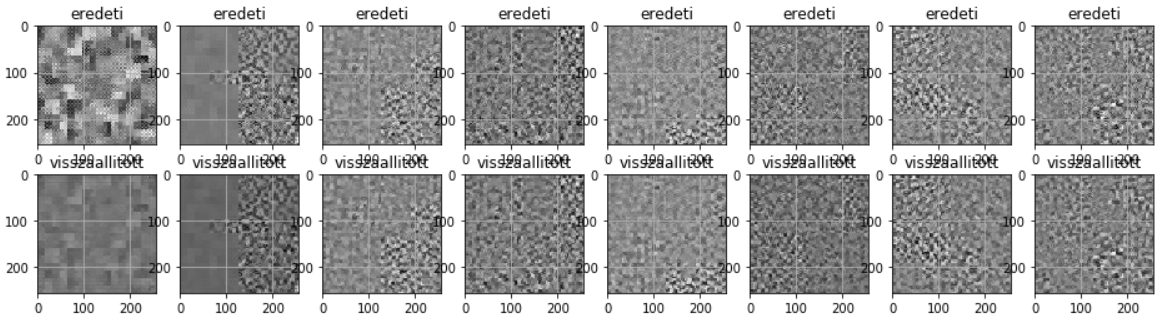
\includegraphics[width=\linewidth]{auto_results.png}
	\caption{Results of the AE with 1st row depicting the input, 2nd row depicting the output.}
	\label{fig:autores}
\end{figure}